\documentclass[t]{beamer}
\usepackage{mathtools}
\usepackage{tikz}
\usepackage{pgfplots}
\usepackage{ulem}
\usetikzlibrary{arrows,backgrounds,shapes,matrix,positioning,fit}
\newcommand{\argmax}{\operatornamewithlimits{argmax}}
\newcommand{\argmin}{\operatornamewithlimits{argmin}}
\newcommand{\wt}{\operatornamewithlimits{wt}}
\newcommand{\var}{\operatornamewithlimits{var}}
\renewcommand\Re{\operatorname{Re}}
\renewcommand\Im{\operatorname{Im}}

\mode<presentation>
{
  \usetheme{Singapore}
  %\useoutertheme{infolines} % Showing only current section in navigation
  \setbeamertemplate{headline}{}  % Empty headline
  \setbeamertemplate{footline}[frame number]  % Getting rid of footer items except slide number
  \setbeamercovered{invisible}
  \beamertemplatenavigationsymbolsempty % Getting rid of navigation bullets at the bottom
}
\usepackage[english]{babel}
\usepackage[latin1]{inputenc}
\usepackage{times}
\usepackage[T1]{fontenc}

\title[EE 703 DMT]{Parameter Estimation}
\author[Saravanan V]
{
  Saravanan Vijayakumaran\\
  \href{mailto:sarva@ee.iitb.ac.in}{sarva@ee.iitb.ac.in}
}
\institute[IIT Bombay]
{
  Department of Electrical Engineering\\
  Indian Institute of Technology Bombay
}
\date{October 21, 2013}

\AtBeginSection[]%
{%
\begin{frame}[plain]%
  \topskip0pt
  \vspace*{\fill}
    \begin{center}%
      \usebeamerfont{section title}\insertsection%
    \end{center}%
  \vspace*{\fill}
\end{frame}%
}

\begin{document}

\begin{frame}
  \titlepage
\end{frame}

\section{Motivation}
%% Frame %%
\begin{frame}{System Model used to Derive Optimal Receivers}
  \footnotesize
  \begin{figure}
    \centering
      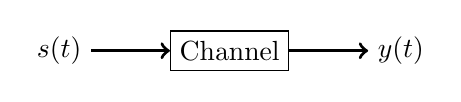
\begin{tikzpicture}[scale=1.0,transform shape]
        \node[rectangle, draw, minimum size = 5mm] (Channel) {Channel};
        \node[left = 1cm of Channel] (st) {$s(t)$};
        \node[right = 1cm of Channel] (rt) {$y(t)$};
        \draw[->,very thick] (st) -- (Channel);
        \draw[->,very thick] (Channel) -- (rt);
      \end{tikzpicture}
  \end{figure}
  \pause
  \begin{equation*}
    y(t) = s(t) + n(t)
  \end{equation*}
  \pause
  \begin{description}
    \item[$s(t)$] Transmitted Signal
    \pause
    \item[$y(t)$] Received Signal
    \pause
    \item[$n(t)$] Noise
  \end{description}
  \pause
  Simplified System Model. \pause Does Not Account For 
  \begin{itemize}
    \item \pause Propagation Delay
    \item \pause Carrier Frequency Mismatch Between Transmitter and Receiver
    \item \pause Clock Frequency Mismatch Between Transmitter and Receiver
  \end{itemize}
  \normalsize
\end{frame}

%% Frame %%
\begin{frame}{Why Study the Simplified System Model?}
  \footnotesize
  \begin{itemize}
    \item \pause Consider the effect of propagation delay
      \begin{figure}
        \centering
          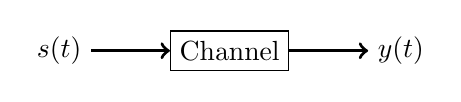
\begin{tikzpicture}[scale=1.0,transform shape]
            \node[rectangle, draw, minimum size = 5mm] (Channel) {Channel};
            \node[left = 1cm of Channel] (st) {$s(t)$};
            \node[right = 1cm of Channel] (rt) {$y(t)$};
            \draw[->,very thick] (st) -- (Channel);
            \draw[->,very thick] (Channel) -- (rt);
          \end{tikzpicture}
      \end{figure}
      \begin{equation*}
        y(t) = s(t - \tau) + n(t)
      \end{equation*}
    \item \pause If the receiver can estimate $\tau$, the simplified system model is valid
    \item \pause Receivers estimate propagation delay, carrier frequency and clock frequency before demodulation
    \item \pause Once these unknown parameters are estimated, the simplified system model is valid
    \item \pause Then why not study parameter estimation first?
      \begin{itemize}
        \footnotesize
        \item \pause Hypothesis testing is easier to learn than parameter estimation
        \item \pause Historical reasons
      \end{itemize}
  \end{itemize}
  \normalsize
\end{frame}

\section{Parameter Estimation}
%% Frame %%
\begin{frame}{Parameter Estimation}
  \footnotesize
  \begin{itemize}
    \item \pause Hypothesis testing was about making a choice between discrete states of nature
    \item \pause Parameter or point estimation is about choosing from a continuum of possible states
  \end{itemize}
  \pause
  \begin{example}[]
    \begin{itemize}
      \item \pause Consider a manufacturer of clothes for newborn babies
      \item \pause She wants her clothes to fit at least 50\% of newborn babies. \pause Clothes can be loose but not tight. \pause She also wants to minimize material used.
      \item \pause Since babies are made up of a large number of atoms, \pause their length is a Gaussian random variable \pause (by Central Limit Theorem)
        \begin{eqnarray*}
          \pause \text{Baby Length} \sim \mathcal{N}(\mu, \sigma^2)
        \end{eqnarray*}
      \item \pause Only knowledge of $\mu$ is required to achieve her goal of 50\% fit
      \item \pause But $\mu$ is unknown and she is interested in estimating it
      \item \pause What is a good estimator of $\mu$? \pause If she wants her clothes to fit at least 75\% of the newborn babies, is knowledge of $\mu$ enough?
    \end{itemize}
  \end{example}
  \normalsize
\end{frame}

%% Frame %%
\begin{frame}{System Model for Parameter Estimation}
  \footnotesize
  \begin{itemize}
    \item \pause Consider a family of distributions
      \begin{equation*}
        \mathbf{Y} \sim P_{\boldsymbol{\theta}}, \ \ \ \boldsymbol{\theta} \in \Lambda
      \end{equation*}
    where the observation vector $\mathbf{Y} \in \Gamma \subseteq \mathbb{R}^n$ and $\Lambda \subseteq \mathbb{R}^m$ is the parameter space. \pause $\boldsymbol{\theta}$ itself can be a realization of a random variable $\boldsymbol{\Theta}$
  \end{itemize}
  \pause
  \begin{example}[]
      \begin{equation*}
        \pause Y \sim \mathcal{N}(\mu, \sigma^2)
      \end{equation*}
    where $\mu$ and $\sigma$ are unknown. \pause Here $\Gamma = \pause \mathbb{R}$, \pause $\boldsymbol{\theta} = \pause \begin{bmatrix} \mu & \sigma \end{bmatrix}^T$, \pause $\Lambda = \pause \mathbb{R}^2$.

      The parameters $\mu$ and $\sigma$ can themselves be random variables.
  \end{example}
  \begin{itemize}
    \item \pause The goal of parameter estimation is to find $\boldsymbol{\theta}$ given $\mathbf{Y}$
    \item \pause An estimator is a function from the observation space to the parameter space
      \begin{equation*}
        \hat{\boldsymbol{\theta}} : \Gamma \rightarrow \Lambda
      \end{equation*}
  \end{itemize} 
  \normalsize
\end{frame}

%% Frame %%
\begin{frame}{Which is the Optimal Estimator?}
  \footnotesize
  \begin{itemize}
    \item \pause Assume there is a cost function $C$
      \begin{equation*}
        C : \Lambda \times \Lambda \rightarrow \mathbb{R}
      \end{equation*}
      such that $C[\mathbf{a},\boldsymbol{\theta}]$ is the cost of estimating the true value of $\boldsymbol{\theta}$ as $\mathbf{a}$
    \item \pause Examples of cost functions for scalar $\theta$
      \begin{description}
        \pause \item[Squared Error] $C[a,\theta] = (a-\theta)^2$
        \pause \item[Absolute Error] $C[a,\theta] = \lvert a - \theta \rvert$ 
        \pause \item[Threshold Error] $C[a,\theta] = \left\{ \begin{array}{cc} 
                                                              0 & \text{if } \lvert a - \theta \rvert \leq \Delta \\
                                                              1 & \text{if } \lvert a - \theta \rvert > \Delta
                                                             \end{array} \right. $
      \end{description}
  \end{itemize}
  \normalsize
\end{frame}

%% Frame %%
\begin{frame}{Which is the Optimal Estimator?}
  \footnotesize
  \begin{itemize}
    \item Suppose that the parameter $\boldsymbol{\theta}$ is the realization of a random variable $\boldsymbol{\Theta}$
    \item \pause With an estimator $\hat{\boldsymbol{\theta}}$ we associate a conditional cost or risk conditioned on $\boldsymbol{\theta}$
      \begin{equation*}
        r_{\boldsymbol{\theta}}(\hat{\boldsymbol{\theta}}) = E_{\boldsymbol{\theta}} \left\{ C\left[\hat{\boldsymbol{\theta}}(\mathbf{Y}), \boldsymbol{\theta} \right]\right\}
      \end{equation*}
    \item \pause The average risk or Bayes risk is given by
      \begin{equation*}
        R(\hat{\boldsymbol{\theta}}) = E\left\{ r_{\boldsymbol{\Theta}}(\hat{\boldsymbol{\theta}})\right\}
      \end{equation*}
    \item \pause The optimal estimator is the one which minimizes the Bayes risk
  \end{itemize}
  \normalsize
\end{frame}

%% Frame %%
\begin{frame}{Which is the Optimal Estimator?}
  \footnotesize
  \begin{itemize}
    \item \pause Given that 
      \begin{eqnarray*}
        r_{\boldsymbol{\theta}}(\hat{\boldsymbol{\theta}}) = E_{\boldsymbol{\theta}} \left\{ C\left[\hat{\boldsymbol{\theta}}(\mathbf{Y}), \boldsymbol{\theta} \right]\right\}
        = E\left\{ C\left[ \hat{\boldsymbol{\theta}}(\mathbf{Y}), \boldsymbol{\Theta} \right]\bigg| \boldsymbol{\Theta} = \boldsymbol{\theta} \right\}
      \end{eqnarray*}
      \pause the average risk or Bayes risk is given by
      \begin{eqnarray*}
        R(\hat{\boldsymbol{\theta}}) & = & E\left\{ C\left[ \hat{\boldsymbol{\theta}}(\mathbf{Y}), \boldsymbol{\Theta} \right]\right\} \\ \pause
                                     & = & E\left\{E\left\{ C\left[ \hat{\boldsymbol{\theta}}(\mathbf{Y}), \boldsymbol{\Theta} \right] \bigg| \mathbf{Y}\right\} \right\} \\ \pause
                                     & = & \int E\left\{ C\left[ \hat{\boldsymbol{\theta}}(\mathbf{Y}), \boldsymbol{\Theta} \right] \bigg| \mathbf{Y} = \mathbf{y}\right\} p_{\mathbf{Y}}(\mathbf{y}) \ d\mathbf{y}
      \end{eqnarray*}
    \item \pause The optimal estimate for $\boldsymbol{\theta}$ can be found by minimizing for each $\mathbf{Y} = \mathbf{y}$ the posterior cost
      \begin{equation*}
        E\left\{ C\left[ \hat{\boldsymbol{\theta}}(\mathbf{y}), \boldsymbol{\Theta} \right] \bigg| \mathbf{Y} = \mathbf{y}\right\} 
      \end{equation*}
  \end{itemize}
  \normalsize
\end{frame}

%% Frame %%
\begin{frame}{Minimum-Mean-Squared-Error (MMSE) Estimation}
  \footnotesize
  \begin{itemize}
    \item \pause Consider a scalar parameter $\theta$
    \item \pause $C[a,\theta] = (a-\theta)^2$
    \item \pause The posterior cost is given by
      \begin{eqnarray*}
        E\left\{ (\hat{\theta}(\mathbf{y}) - \Theta)^2 \bigg| \mathbf{Y} = \mathbf{y}\right\} & = & \pause \left[ \hat{\theta}(\mathbf{y})\right]^2 \\
                                                                                     &   & - 2\hat{\theta}(\mathbf{y}) E\left\{ \Theta \bigg| \mathbf{Y} = \mathbf{y}\right\} \\
                                                                                     &   & + E \left\{ \Theta^2 \bigg| \mathbf{Y} = \mathbf{y}\right\}
      \end{eqnarray*}
    \item \pause Differentiating posterior cost wrt $\hat{\theta}(\mathbf{y})$, the Bayes estimate is  \pause
      \begin{equation*}
        \hat{\theta}_{MMSE}(\mathbf{y}) = E\left\{ \Theta \bigg| \mathbf{Y} = \mathbf{y} \right\}
      \end{equation*}
  \end{itemize}
  \normalsize
\end{frame}

%% Frame %%
\begin{frame}{Example: MMSE Estimation}
  \footnotesize
  \begin{itemize}
    \item \pause Suppose $X$ and $Y$ are jointly Gaussian random variables
    \item \pause Let the joint pdf be given by
      \begin{equation*}
        p_{XY}(x,y) = \frac{1}{2\pi \lvert \mathbf{C} \rvert^{\frac{1}{2}}} \exp\left( -\frac{1}{2}(\mathbf{s} - \boldsymbol{\mu})^T\mathbf{C}^{-1}(\mathbf{s}-\boldsymbol{\mu})\right)
      \end{equation*}
    where $\mathbf{s} = \begin{bmatrix} x \\ y \end{bmatrix}$, $\boldsymbol{\mu} = \begin{bmatrix} \mu_x \\ \mu_y \end{bmatrix}$ and $\mathbf{C} = \begin{bmatrix} \sigma_x^2 & \rho \sigma_x \sigma_y \\ \rho \sigma_x \sigma_y & \sigma_y^2\end{bmatrix}$
    \item \pause Suppose $Y$ is observed and we want to estimate $X$
    \item \pause The MMSE estimate of $X$ is 
      \begin{equation*}
        \hat{X}_{MMSE}(y) = E\left[X \bigg| Y = y \right]
      \end{equation*}
    \item \pause The conditional density of $X$ given $Y = y$ is
      \begin{equation*}
        p(x|y) = \frac{p_{XY}(x,y)}{p_Y(y)}
      \end{equation*}
  \end{itemize}
  \normalsize
\end{frame}

%% Frame %%
\begin{frame}{Example: MMSE Estimation}
  \footnotesize
  \begin{itemize}
    \item The conditional density of $X$ given $Y=y$ is a Gaussian density with mean
      \begin{equation*}
        \mu_{X|y} = \mu_x + \frac{\sigma_x}{\sigma_y}\rho(y-\mu_y)
      \end{equation*}
      \pause and variance
      \begin{equation*}
        \sigma^2_{X|y} = (1-\rho^2)\sigma_x^2
      \end{equation*}
    \item \pause Thus the MMSE estimate of $X$ given $Y = y$ is
      \begin{equation*}
        \hat{X}_{MMSE}(y) = \mu_x + \frac{\sigma_x}{\sigma_y}\rho(y-\mu_y)
      \end{equation*}
  \end{itemize}
  \normalsize
\end{frame}

%% Frame %%
\begin{frame}{Maximum A Posteriori (MAP) Estimation}
  \footnotesize
  \begin{itemize}
    \item \pause In some situations, the conditional mean may be difficult to compute
    \item \pause An alternative is to use MAP estimation
    \item \pause The MAP estimator is given by
      \begin{equation*}
        \hat{\boldsymbol{\theta}}_{MAP}(\mathbf{y}) = \argmax_{\boldsymbol{\theta}} p\left(\boldsymbol{\theta} | \mathbf{y}\right)
      \end{equation*}
      where $p$ is the conditional density of $\boldsymbol{\Theta}$ given $\mathbf{Y}$.
    \item \pause It can be obtained as the optimal estimator for the threshold cost function
      \begin{equation*}
        C[a,\theta] = \left\{ \begin{array}{cc} 
                                                              0 & \text{if } \lvert a - \theta \rvert \leq \Delta \\
                                                              1 & \text{if } \lvert a - \theta \rvert > \Delta
                                                             \end{array} \right. 
      \end{equation*}
      for small $\Delta > 0$
  \end{itemize}
  \normalsize
\end{frame}

%% Frame %%
\begin{frame}{Maximum A Posteriori (MAP) Estimation}
  \footnotesize
  \begin{itemize}
    \item For the threshold cost function, we have\footnote{Assume a scalar parameter $\theta$ for illustration} 
      \begin{eqnarray*}
        \lefteqn{E\left\{ C\left[ \hat{\theta}(\mathbf{y}), \Theta \right] \bigg| \mathbf{Y} = \mathbf{y}\right\}} \\
           & = & \pause \int_{-\infty}^{\infty} C[\hat{\theta}(\mathbf{y}), \theta] p\left(\theta| \mathbf{y}\right) \ d\theta \\
           & = & \pause \int_{-\infty}^{\hat{\theta}(\mathbf{y})-\Delta} p\left(\theta| \mathbf{y}\right) \ d\theta + \int_{\hat{\theta}(\mathbf{y})+\Delta}^{\infty} p\left(\theta| \mathbf{y}\right) \ d\theta\\
           & = & \pause \int_{-\infty}^{\infty} p\left(\theta| \mathbf{y}\right) \ d\theta - \int_{\hat{\theta}(\mathbf{y})-\Delta}^{\hat{\theta}(\mathbf{y})+\Delta} p\left(\theta| \mathbf{y}\right) \ d\theta\\
           & = & \pause 1  - \int_{\hat{\theta}(\mathbf{y})-\Delta}^{\hat{\theta}(\mathbf{y})+\Delta} p\left(\theta| \mathbf{y}\right) \ d\theta
      \end{eqnarray*}
    \item \pause The Bayes estimate is obtained by maximizing the integral in the last equality
  \end{itemize}
  \normalsize
\end{frame}

%% Frame %%
\begin{frame}{Maximum A Posteriori (MAP) Estimation}
  \footnotesize
    \begin{figure}
      \centering
        \begin{tikzpicture}[scale=0.50,transform shape]
          \begin{axis}[
                       xmax=5.9,
                       xmin=-5.9,
                       ymax=0.3,
                       ymin=-0.01,
                       axis x line = middle,
                       axis y line = left,
                       xtick = {-1.25},
                       xticklabels = {$\hat{\theta}(\mathbf{y})$},
                       ytick={0.295},
                       yticklabels = {$p(\theta |  \mathbf{y})$},
                       legend style = {font = \tiny},
                       x post scale = 2.0
                      ]
                \addplot[color=blue,fill=blue,fill opacity=0.5,area legend,very thick,domain=-1.5:-1,samples=100] gnuplot{exp(-(x)*(x)/(2*2))/sqrt(2*pi*2)} \closedcycle;
                \addlegendentry{$\int_{\hat{\theta}(\mathbf{y})-\Delta}^{\hat{\theta}(\mathbf{y})+\Delta} p\left(\theta|\mathbf{y}\right)$}
                \addplot[color=blue,very thick,domain=-6:6,samples=100] gnuplot{exp(-(x)*(x)/(2*2))/sqrt(2*pi*2)};
          \end{axis}
        \end{tikzpicture}
    \end{figure}
  \begin{itemize}
    \item The shaded area is the integral $\int_{\hat{\theta}(\mathbf{y})-\Delta}^{\hat{\theta}(\mathbf{y})+\Delta} p\left(\theta|\mathbf{y}\right)\ d\theta$
    \item \pause To maximize this integral, the location of $\hat{\theta}(\mathbf{y})$ should be chosen to be the value of $\theta$ which maximizes $p(\theta | \mathbf{y})$
  \end{itemize}
  \normalsize
\end{frame}

%% Frame %%
\begin{frame}{Maximum A Posteriori (MAP) Estimation}
  \footnotesize
    \begin{figure}
      \centering
        \begin{tikzpicture}[scale=0.50,transform shape]
          \begin{axis}[
                       xmax=5.9,
                       xmin=-5.9,
                       ymax=0.3,
                       ymin=-0.01,
                       axis x line = middle,
                       axis y line = left,
                       xtick = {0},
                       xticklabels = {$\hat{\theta}_{MAP}(\mathbf{y})$},
                       ytick={0.295},
                       yticklabels = {$p(\theta | \mathbf{y})$},
                       legend style = {font = \tiny},
                       x post scale = 2.0
                      ]
                \addplot[color=blue,fill=blue,fill opacity=0.5,area legend,very thick,domain=-0.25:0.25,samples=100] gnuplot{exp(-(x)*(x)/(2*2))/sqrt(2*pi*2)} \closedcycle;
                \addlegendentry{$\int_{\hat{\theta}(\mathbf{y})-\Delta}^{\hat{\theta}(\mathbf{y})+\Delta} p\left(\theta| \mathbf{y}\right)$}
                \addplot[color=blue,very thick,domain=-6:6,samples=100] gnuplot{exp(-(x)*(x)/(2*2))/sqrt(2*pi*2)};
          \end{axis}
        \end{tikzpicture}
    \end{figure}
  \begin{itemize}
    \item \pause This argument is not airtight as $p(\theta | \mathbf{y})$ may not be symmetric at the maximum
    \item \pause But the MAP estimator is widely used as it is easier to compute than the MMSE estimator
  \end{itemize}
  \normalsize
\end{frame}

%% Frame %%
\begin{frame}{Maximum Likelihood (ML) Estimation}
  \footnotesize
  \begin{itemize}
    \item \pause The ML estimator is given by
      \begin{equation*}
        \hat{\boldsymbol{\theta}}_{ML}(\mathbf{y}) = \argmax_{\boldsymbol{\theta}} p\left(\mathbf{y} | \boldsymbol{\theta}\right)
      \end{equation*}
      where $p$ is the conditional density of $\mathbf{Y}$ given $\boldsymbol{\Theta}$.
    \item \pause It is the same as the MAP estimator when the prior probability distribution of $\boldsymbol{\Theta}$ is uniform
      \begin{equation*}
        \hat{\boldsymbol{\theta}}_{MAP}(\mathbf{y}) = \argmax_{\boldsymbol{\theta}} p\left(\boldsymbol{\theta} | \mathbf{y}\right) = \pause \argmax_{\boldsymbol{\theta}} \frac{p\left(\boldsymbol{\theta}, \mathbf{y}\right)}{p(\mathbf{y})} = \pause \argmax_{\boldsymbol{\theta}} \frac{p\left(\mathbf{y}|\boldsymbol{\theta}\right)p(\boldsymbol{\theta})}{p(\mathbf{y})}
      \end{equation*}
    \item \pause It is also used when the prior distribution is not known
  \end{itemize}
  \normalsize
\end{frame}

%% Frame %%
\begin{frame}{Example 1: ML Estimation}
  \footnotesize
  \begin{itemize}
    \item \pause Suppose we observe $Y_i, \ i=1,2,\ldots,M$ such that 
      \begin{equation*}
        Y_i \sim \mathcal{N}(\mu, \sigma^2)
      \end{equation*}
      where $Y_i$'s are independent, $\mu$ is unknown and $\sigma^2$ is known
    \item \pause The ML estimate is given by
      \begin{equation*}
        \hat{\mu}_{ML}(\mathbf{y}) = \pause \frac{1}{M} \sum_{i=1}^M y_i
      \end{equation*}
  \end{itemize}
  \normalsize
\end{frame}

%% Frame %%
\begin{frame}{Example 2: ML Estimation}
  \footnotesize
  \begin{itemize}
    \item \pause Suppose we observe $Y_i, \ i=1,2,\ldots,M$ such that 
      \begin{equation*}
        Y_i \sim \mathcal{N}(\mu, \sigma^2)
      \end{equation*}
      where $Y_i$'s are independent, both $\mu$ and $\sigma^2$ are unknown
    \item \pause The ML estimates are given by
      \begin{eqnarray*}
        \hat{\mu}_{ML}(\mathbf{y}) & = & \pause \frac{1}{M} \sum_{i=1}^M y_i \\ \pause
        \hat{\sigma}^2_{ML}(\mathbf{y}) & = & \pause \frac{1}{M} \sum_{i=1}^M \left(y_i - \hat{\mu}_{ML}(\mathbf{y})\right)^2
      \end{eqnarray*}
  \end{itemize}
  \normalsize
\end{frame}

%% Frame %%
\begin{frame}{Example 3: ML Estimation}
  \footnotesize
  \begin{itemize}
    \item \pause Suppose we observe $Y_i, \ i=1,2,\ldots,M$ such that 
      \begin{equation*}
        Y_i \sim \text{Bernoulli}(p)
      \end{equation*}
      where $Y_i$'s are independent and $p$ is unknown
    \item \pause The ML estimate of $p$ is given by
      \begin{eqnarray*}
        \hat{p}_{ML}(\mathbf{y}) =  \pause \frac{1}{M} \sum_{i=1}^M y_i 
      \end{eqnarray*}
  \end{itemize}
  \normalsize
\end{frame}

%% Frame %%
\begin{frame}{Example 4: ML Estimation}
  \footnotesize
  \begin{itemize}
    \item \pause Suppose we observe $Y_i, \ i=1,2,\ldots,M$ such that 
      \begin{equation*}
        Y_i \sim \text{Uniform}[0,\theta]
      \end{equation*}
      where $Y_i$'s are independent and $\theta$ is unknown
    \item \pause The ML estimate of $\theta$ is given by
      \begin{eqnarray*}
        \hat{\theta}_{ML}(\mathbf{y}) =  \pause \max\left(y_1,y_2,\ldots,y_{M-1},y_M \right)
      \end{eqnarray*}
  \end{itemize}
  \normalsize
\end{frame}

%% Frame %%
\begin{frame}{Reference}
  \begin{itemize}
    \item  Chapter 4, \textit{An Introduction to Signal Detection and Estimation}, H.~V.~Poor, Second Edition, Springer Verlag, 1994.
  \end{itemize}
\end{frame}

%% Frame %%
\begin{frame}{}
\vfill
\begin{center}
Thanks for your attention
\end{center}
\vfill
\end{frame}

\end{document}
